\documentclass[10pt,a4paper]{article}
\usepackage[utf8]{inputenc}
\usepackage[french]{babel}
\usepackage[T1]{fontenc}
\usepackage{amsmath}
\usepackage{amsfonts}
\usepackage{amssymb}
\usepackage{amsthm}
\usepackage{bbold}

\usepackage{graphicx}

\theoremstyle{definition}
\newtheorem{definition}{Definition}
\theoremstyle{definition}
\newtheorem{theorem}{Theorem}
\theoremstyle{definition}
\newtheorem{notation}{Notation}

\author{Della Bona Sarah, Dumez Erika}
\title{Introduction to neural ODE}
\begin{document}
\maketitle

\section{Introduction}

In this document, we introduce ODE-nets, which are deep neural networks models using ordinary differential equations. We focus in particular on the mathematical aspects of these neural networks. We will give definitions and properties for different notions such as ordinary differential equations, regular and residual neural networks, implicit layers, ... 

\noindent At the end, we'll conclude with the advantages and disadvantages of ODE-nets.


\section{Ordinary Differential Equations}

\subsection{A reminder on ordinary differential equations}

An ordinary differential equation, noted "ODE", is an equation that describes the changes of a function through time. The aim is to compute that function from the ODE which describes its derivative. In this setting, time is a continuous variable.


\begin{notation}
Let $f: \mathbb{R}^n \rightarrow \mathbb{R}^m$ be a function.

We denote the derivative of $f$ as :
$$
\partial f : \mathbb{R}^n \rightarrow \mathbb{R}^m
$$

We also write, for $x \in \mathbb{R}^n$ :
$$
\partial_t f(x) = \frac{\partial f(x)}{\partial t} 
$$
\end{notation}

\begin{definition}
Let $\Omega \subseteq \mathbb{R} \times \mathbb{R}^N$ an open set. Let $f: \Omega \rightarrow \mathbb{R}^N$. 

A \textit{first order ODE} takes of the form:
$$
\partial_t u(t) = f(t,u(t))
$$

\begin{itemize}
%TODO Définir d'où vient le I ?
\item A \textit{solution} for this ODE is a function $u : I \rightarrow \mathbb{R}^N$ where $I$ is an interval of $\mathbb{R}$ such that:
	\begin{itemize}
	\item[•] u is derivable on I,
	\item[•] $\forall t \in I, (t, u(t)) \in \Omega$,
	\item[•] $\forall t \in I, \partial_t u(t) = f(t, u(t))$
	\end{itemize}
~

\item An \textit{initial condition} (IC) is a condition of the type:
$$
u(t_0) = u_0
$$
where $(t_0, u_0) \in \Omega$ is fixed.

~

\item A \textit{Cauchy problem} is an ODE with IC :
$$
\left \{
\begin{array}{rcl}
\partial_t u(t) & = & f(t, u(t)) \\
u(t_0) & = & u_0
\end{array}
\right.
$$
\end{itemize}
\end{definition}

\begin{definition}
A \textit{k-order ODE}, with $k \in \mathbb{N}\backslash \{0\}$, takes the form:
$$
\partial^k_t v(t) = g(t, v(t), ... , \partial^{k-1}v(t))
$$
where 

\begin{align*}
v &:  I \rightarrow \mathbb{R}^N, I\subset \mathbb{R} \\ 
g &:  \Theta \subseteq \mathbb{R} \times \mathbb{R}^N \times ... \times \mathbb{R}^N \rightarrow \mathbb{R}^N
\end{align*} 
\end{definition}

\subsection{A simple example}
Let $\partial_t x(t) = x(t)$ an ODE. The solutions of this ODE are given by : 
$$
a . e^t \text{ where } a\in \mathbb{R}.
$$

Indeed, we have:
$$
\partial_t a.e^t = a.e^t
$$
If we add an initial condition $x(0) = 1$, we have a Cauchy problem and its solution is $e^t$, since $e^0 = 1$ and $\partial_te^t = e^t$.

\subsection{Existence and uniqueness of a solution}

If we want to calculate a function from an ODE, we need to know the conditions under which this ODE has a solution. Thus, we define \textit{Lipschitz continuous functions}. This notion is crucial for the following theorem which gives conditions for the existence and uniqueness of a solution to an ODE.

\begin{definition}
Let $(X, d_X)$ and $(Y, d_Y)$ be two metric spaces.  

A function $f: X \rightarrow  Y$ is called \textit{Lipschitz continuous} if
$$
\exists K \geq 0, \  \forall x_1, x_2 \in X, \  d_Y(f(x_1), f(x_2)) \leq Kd_X(x_1, x_2).
$$
\end{definition}

\begin{theorem}{\textbf{Picard-Lindelöf theorem}}

Consider the Cauchy problem :
$$
y'(t) = f(t, y(t)), \ \ \ y(t_0) = y_0.
$$
Suppose $f$ is uniformly Lipschitz continuous in $y$ and continuous in $t$. Then for some value $\epsilon > 0$, there exists a unique solution $y(t)$ to the Cauchy problem on the interval $[t_0 - \epsilon, t_0 + \epsilon]$. 
\end{theorem}

\subsection{Euler's method}
Unfortunately, as we saw in the previous theorem, it is not always possible to explicitly find a solution to a Cauchy problem. However, we can compute a finite number of points $u_i \in \mathbb{R}^N$ which are close to the real solution and thus, approximate the real function. 

More precisely, let $T \in \mathbb{R}\backslash\{0\}$ such that the solution $u$ exists on $[t_0, t_0 + T]$ and let $n \in \mathbb{N}^{\geqslant 2}$. We are then looking for $(u_i)^n_{i=0}$ such that:
$$
u_i \approx u(t_i) \ \text{ where } t_0 < ... < t_n \in [t_0, t_0 + T]
$$

To compute those points, we use \textit{1-step methods}. These methods compute the points $u_{i+1}$ from the previous point $u_i$, the time $t_i$ and the \textit{step} $h_i := t_{i+1} - t_i$.

Euler's method is a 1-step method with a constant step $h$. It is similar to a Taylor development: the idea is to compute $u(t_{i+1})$ using the following formula:
$$
u(t_{i+1}) \approx u(t_i) + h . \partial u(t_i)
$$
where 
$$
\partial u(t_i) = f(t_i, u(t_i)).
$$

\begin{definition}
Let $f: \mathbb{R}^n \rightarrow \mathbb{R}^m$ be a function.

We can write the \textit{first-order Taylor's development} for $f$ at $x$ as :
$$
f(x + a) = f(x) + a . \partial f(x) + O(\| a\|^2)
$$

where $a \in \mathbb{R}^n$ is a vector.
\end{definition}

\section{Neural networks}

In a typical machine learning problem, we are given some input $x$ and we want to predict an output $y$. 

\noindent A \textit{neural network} can be used to solve such a problem. It consists of a series of layers. There are three types of layers :

\begin{itemize}
\item The \textit{input} layer
\item The \textit{output} layer
\item The \textit{hidden} layers
\end{itemize}

Each layer consist of a certain number of neurons. We give an input to the neurons of a layer, they do some calculus and give an output. An \textit{activation function} is then applied to this output before transmitting it to the next layer thanks to the connections between the neurons of each layer.

~

We begin by giving an input to the input layer, which transmits information to the first hidden layer\footnote{There isn't always an hidden layer in a neural network}. In turn, it transmit information to the next layer and so on, until the output layer gives us the final output, the \textit{prediction}. An example of neural network is given in figure \ref{examplenn}.

\begin{figure}
\center
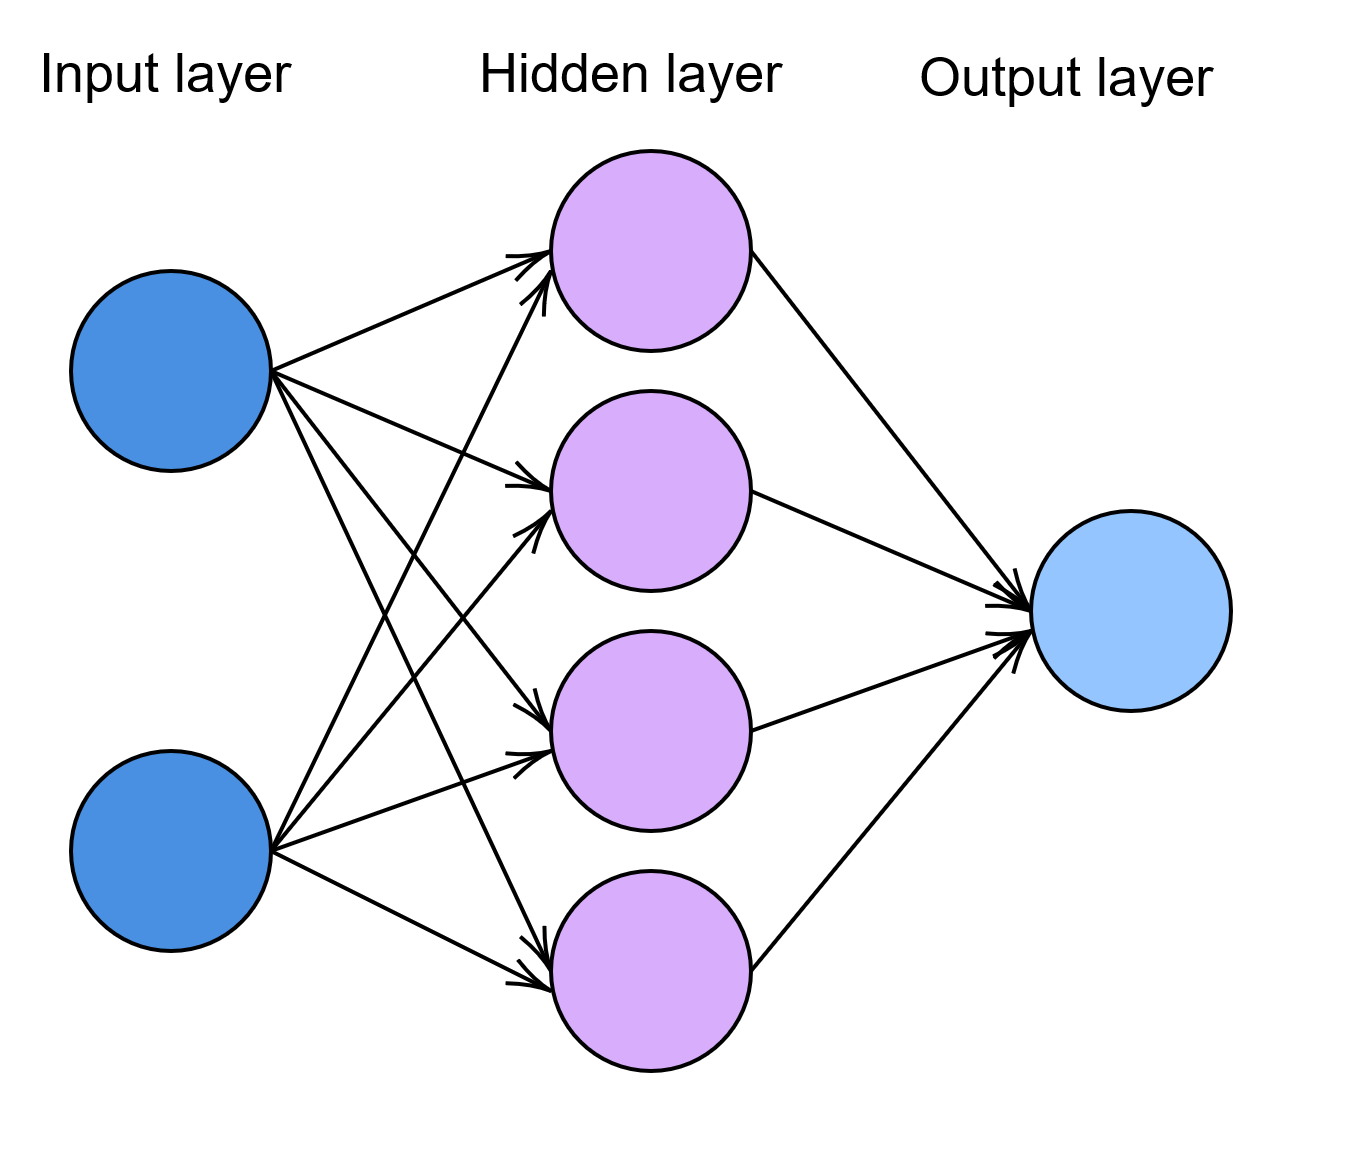
\includegraphics[scale=0.2]{nn.png}
\caption{Example of neural network}
\label{examplenn}
\end{figure}

\newpage

To evaluate the accuracy of a neural network, we use \textit{loss functions.} 

Let $x$ be an input for our neural network. A loss function $L$ takes as input the prediction of the network for $x$ and the real output $y$ of that input $x$, and returns a real value which represents the error for that input. 

An example of loss function for outputs in $\mathbb{R}$ is the function that returns $|y - f(x)|$, where $x$ is the input, $y$ is its associated output and $f(x)$ is the output predicted by the network.

The goal is to minimize this error for every input. To do that, we need to find the optimal parameters for the network which minimize this loss function.

\subsection{Example} \label{exnn}
Let's consider a neural network with one hidden layer that takes a 2 - dimensional input $x = (x_1, x_2)$ and gives a 2-dimensional output $y = (y_1,y_2)$. We can represent this network with the following equations:

\begin{eqnarray*}
z_i = \sum_{j=1}^2 w_{ij}^{(1)}x_j + b_i^{(1)} & \text{ pour } i = 1,2 \\ 
h_i = \sigma (z_i) & \text{ pour } i=1,2 \\
y_k = \sum_{i=1}^2 w_{ki}^{(2)}h_i + b_k^{(2)} & \text{ pour } k = 1,2 \\
\mathcal{L} = \frac{1}{2} \sum_{k = 1}^2 (y_k - t_k)^2
\end{eqnarray*}
   
where $w^{(1)}$, $w^{(2)}$, $b^{(1)}$ and $b^{(2)}$ are parameters of the network and $t = (t_1, t_2)$ is the value we want to approximate (the "real" output for $x$). 

In this network, the first layer takes as input $x_i$ and returns $h_i = \sigma(z_i)$. This value is given to the next layer, which is actually the output layer. The final output is then $y_i$.

\subsection{Back propagation}
%TODO donner le théorème ou le truc qui dis que pour trouver le minimum d'une fonction on
%doit trouver la valeur qui annule la dérivée?
To find the parameters that minimize the loss function, we need to determine the differential of the loss function with respect to the parameters. This process is called \textit{backpropagation}.

For the previous example, we have:
\begin{eqnarray*}
\frac{\partial \mathcal{L}}{\partial \mathcal{L}} & = & 1 \\
\frac{\partial \mathcal{L}}{\partial y_k} & = & \frac{\partial \mathcal{L}}{\partial \mathcal{L}} . (y_k - t_k) \\
\frac{\partial \mathcal{L}}{\partial w_{ki}^{(2)}} & = & \frac{\partial \mathcal{L}}{\partial y_k} . h_i \\
\frac{\partial \mathcal{L}}{\partial b_k^{(2)}} & = & \frac{\partial \mathcal{L}}{\partial y_k} \\
\frac{\partial \mathcal{L}}{\partial h_i} & = & \sum_{k = 1}^2 \frac{\partial \mathcal{L}}{\partial y_k} . w_{ki}^{(2)} \\
\frac{\partial \mathcal{L}}{\partial z_i} & = & \frac{\partial \mathcal{L}}{\partial h_i} \sigma '(z_i) \\
\frac{\partial \mathcal{L}}{\partial w_{ij}^{(1)}} & = & \frac{\partial \mathcal{L}}{\partial z_i} . x_j \\
\frac{\partial \mathcal{L}}{\partial b_i^{(1)}} & = & \frac{\partial \mathcal{L}}{\partial z_i} \\
\end{eqnarray*}

%TODO ajouter computation graph + methode vectorielle ?

\section{Residual neural network} \label{rnn}

A deep neural network really close the a neural ODE network is the \textit{residual neural network}, also called ResNet. It is simply a regular neural network except that it has more connections. Not only do we feed the output of the previous layer to the next, but also the input of that layer. 
An example of the representation of a ResNet is given in figure \ref{exampleresnet}

In these networks, the $k+1$th layer has the formula:
$$
x_{k+1} = x_k + F(x_k)
$$
where $F$ is the function of the $k$th layer and its activation. 

We can see that this simple formula is a special case of the formula:
$$
x_{k+1} = x_k + h.F(x_k),
$$
which is the formula for the Euler method for solving ODEs when $h = 1$. It is with this observation that we can later introduce neural ODE networks.

\begin{figure}
\center
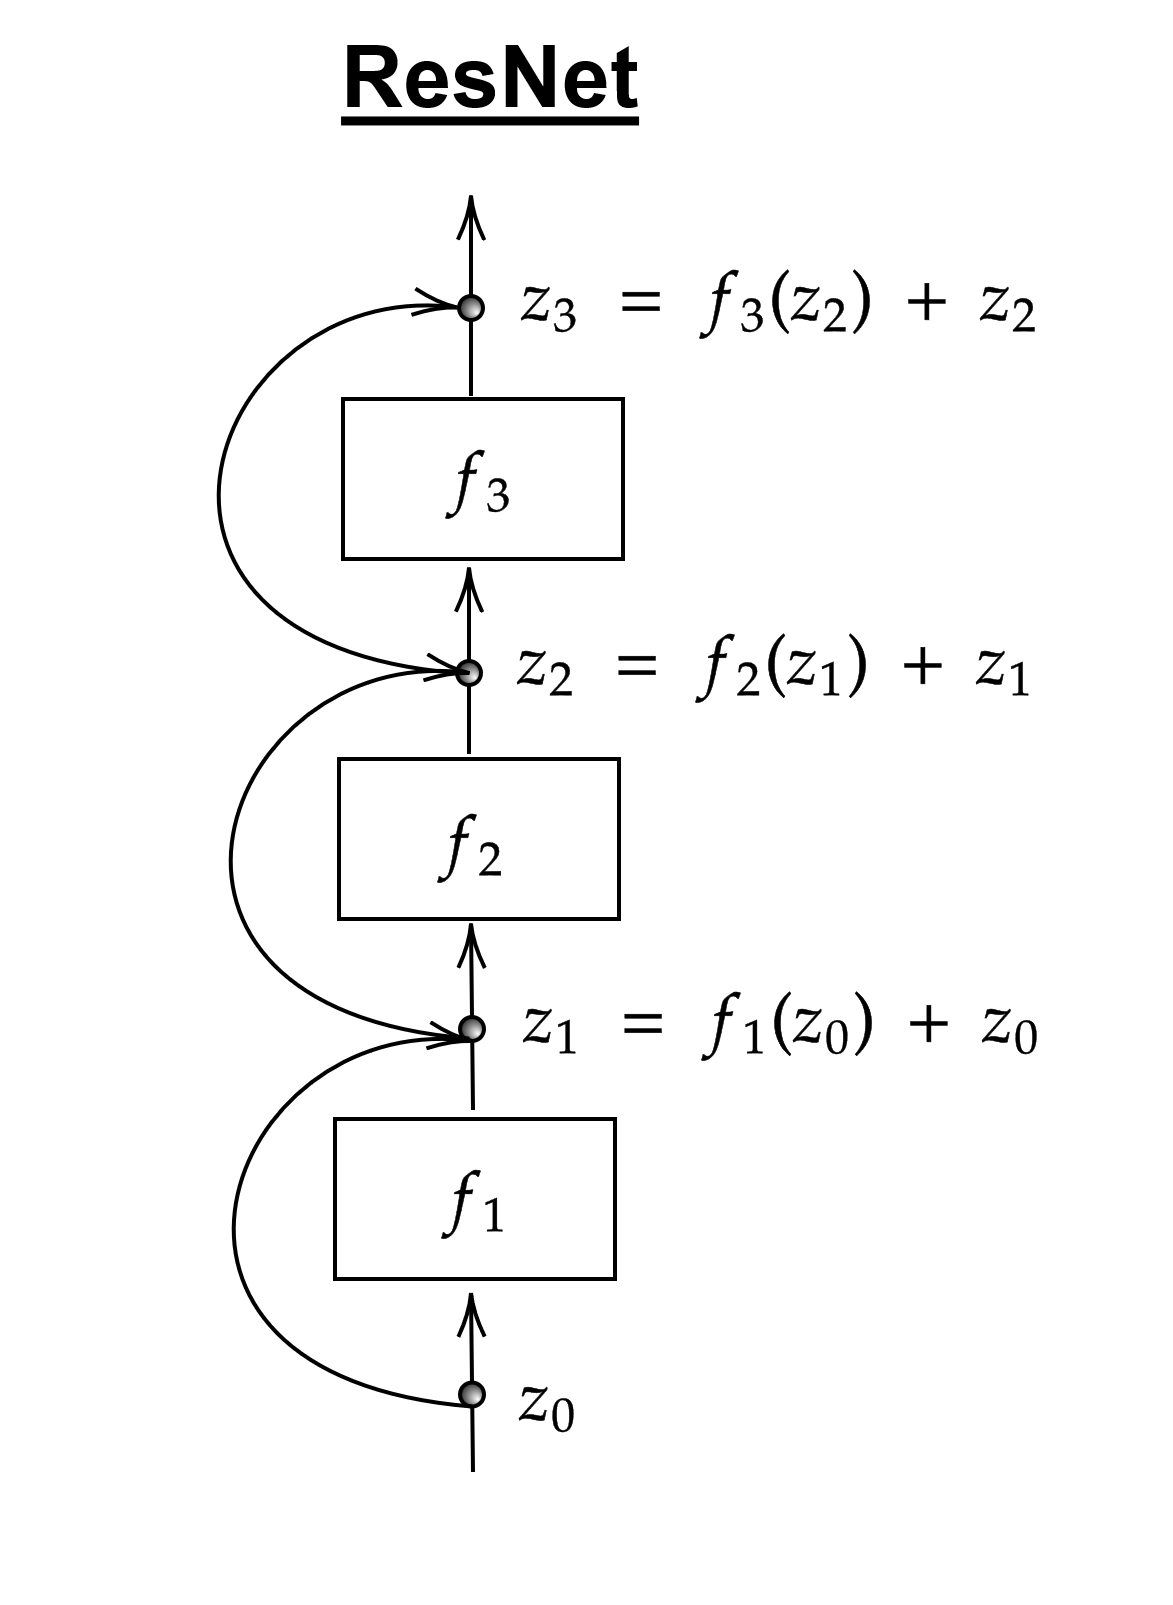
\includegraphics[scale=0.18]{resnet.png}
\caption{Example of residual neural network}
\label{exampleresnet}
\end{figure}

~

With these additional connections, we can avoid the problems of the \textit{vanishing gradient} and the \textit{exploding gradient} and thus have a better accuracy. 

The vanishing gradient problem is encountered when using gradient descent in the backpropagation. Each of the neural network's weights receives an update proportional to the partial derivative of the loss function with respect to the current weight in each iteration of training. 

The problem is that in some cases, the gradient will be vanishingly small, effectively preventing the weight from changing its value. Given that these partial derivatives are computed with the chain rule, this can easily occur, because you keep on multiplying small numbers. The deeper is the neural network, the more likely this problem can occur. In the worst case, this may completely stop the neural network from further training. 

When the derivatives take on larger values, then we have the opposite problem, the exploding gradient problem.

Residual networks avoid the problem of vanishing gradient by introducing short paths which can carry a gradient over the entire extent of very deep networks. This is because adding the information from the previous layer will make these activations larger, so to some extent, they will prevent these activations from becoming exponentially small.

%TODO regarder à la première vidéo pour explications sur pourquoi ça empêche ce problème

\section{Implicit Layers}

There is two different ways to define a layer : \textit{explicitly} or \textit{implicitly}. When we define a layer explicitly, we specify the exact sequence of operations to do from the input to the output layer like in the example of the section \ref{exnn}. 

However, when we add some functionality to the layers, it can become complex to define them explicitly. Instead, we can define them implicitly: we specify the condition we want the layer's output to satisfy. 

Formally, let's assume that we have an input space $\mathcal{X}$ and an output space $\mathcal{Y}$. An explicit layer is defined by a function $f : \mathcal{X} \rightarrow \mathcal{Y}$. 

~

For an implicit layer, we give a condition that a function $g: \mathcal{X} \times \mathcal{Y} \rightarrow \mathbb{R}^n$ should satisfy. For example we can search for a $y$ such that $g(x,y) = 0$.


%A special case is a layer that uses an ODE solver. For each layer $t$ we define the output $y(t)$ as %the solution of the ODE:
%$$
%\partial_t y(t) = f(t, y(t)), \qquad y(0) = y_0.
%$$

\subsection{Implicit function theorem}

Sometimes, variables can not be defined by a function but are rather defined by an equation. In this case, the \textit{implicit function theorem} can be used. It says that if a function $f$ is sufficiently regular in the neighborhood of a point, then there exists a function $\varphi$ at least as regular as $f$ such that locally, the graph of $f$ and the graph of $\varphi$ are the same.

\begin{theorem}{\textbf{The implicit function theorem}}

Let $f: \mathbb{R}^p \times \mathbb{R}^n \rightarrow \mathbb{R}^n$ be a function and $a_0 \in \mathbb{R}^p , z_0 \in \mathbb{R}^n$ two vectors such that :

\begin{enumerate}
\item $f(a_0,z_0) = 0$;
\item $f$ is continuously differentiable with a non-singular Jacobian, i.e. its determinant is non zero, $\partial_z f(a_0,z_0) \in \mathbb{R}^{n \times n}$.
\end{enumerate}
Then there exist open sets $S_{a_0} \subset \mathbb{R}^p$ and $S_{z_0} \subset \mathbb{R}^n$ containing $a_0$ and $z_0$, respectively, and a unique continuous function $z*:S_{a_0} \rightarrow S_{z_0}$ such that:
\begin{itemize}
\item $z_0=z^*(a_0)$,
\item $ \forall a \in S_{a_0}, f(a,z^*(a))=0$,
\item $z^*$ is differentiable on $S_{a_0}$.
\end{itemize}
\end{theorem}

We could use the theorem to compute the derivatives for the backpropagation, but in the following we will use a simpler derivation based on ResNet with the adjoint method.

\section{Neural ODE}

\subsection{Définition}

%TODO voir def vector field

In a residual neural network, the output for an input $x$ is a composition of functions $F(x, \theta)$ where $\theta$ represents the parameters of the layers. 

We want to extract all these individual layers to only have one "shared" layer.

A \textit{neural ODE network} (or ODE-Net) takes a simple layer as a building block. This “base layer” is going to specify the dynamics of an ODE.
ODE-Net enable us to replace layers of neural networks with a continuous-depth model. This means that we do not need to specify the number of layers beforehand.

Let's return to ResNets to give intuition behind this definition.
We know that any output of a layer of a residual network can be computed with the function:
$$F(z_t, t, \theta) = f(z_t, t) + z_t$$
with $t$ being the layer's number minus one.

\begin{figure}
\center
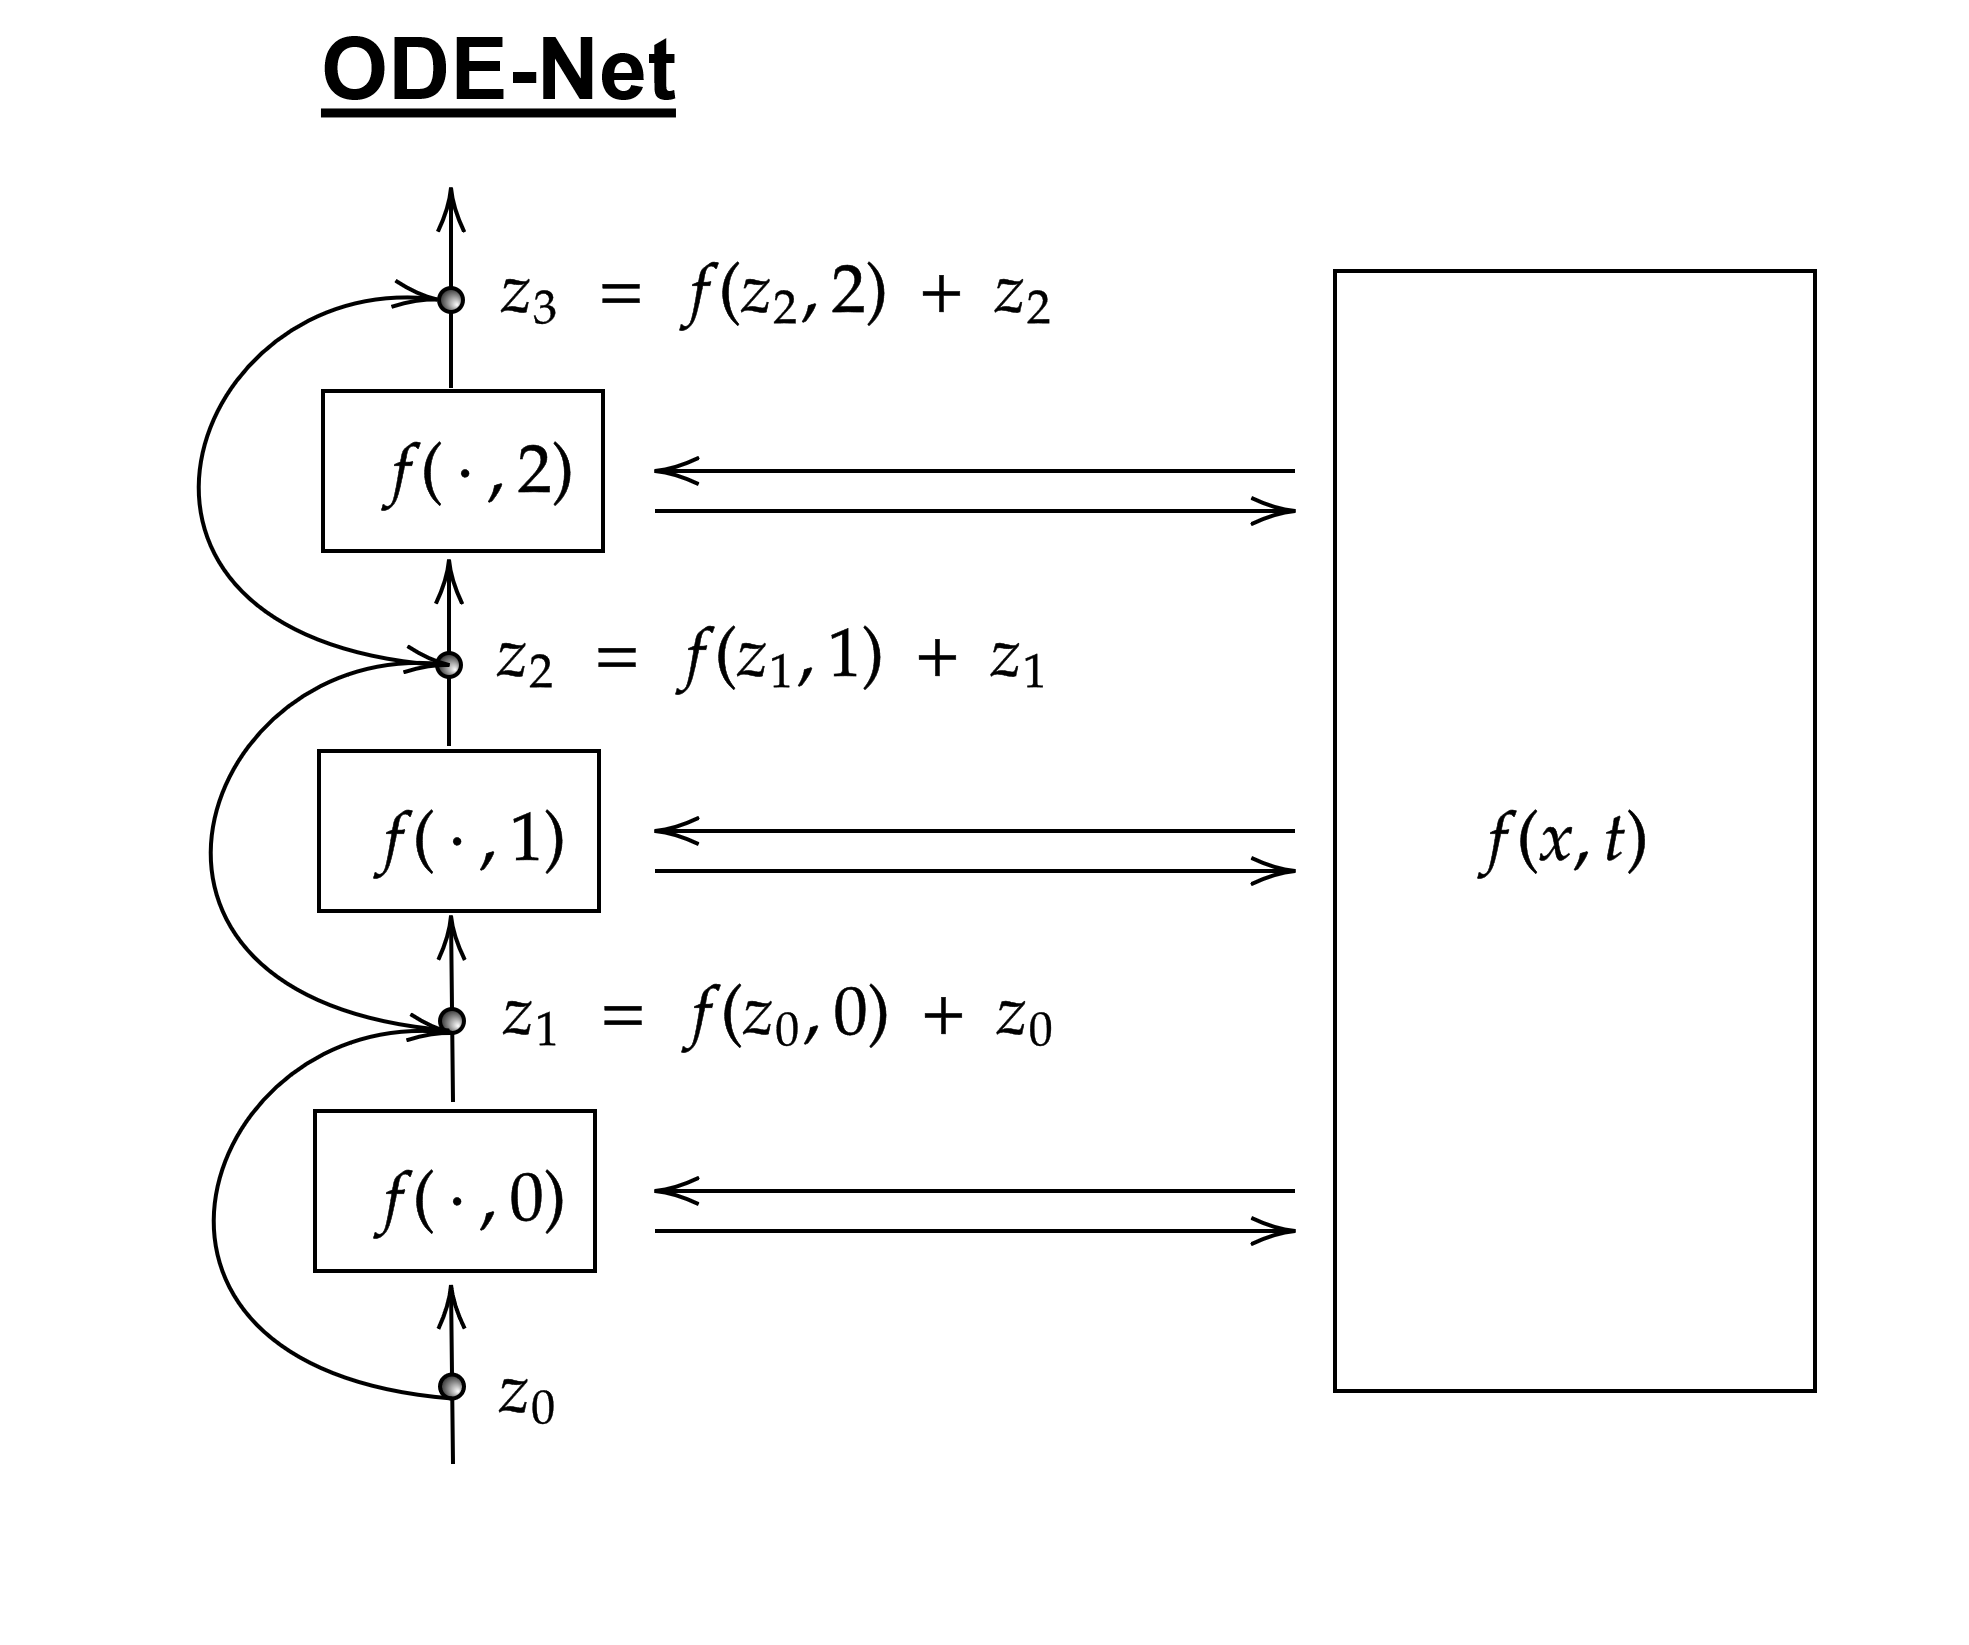
\includegraphics[scale=0.18]{ODENet.png}
\caption{Representation of an ODE-Net}
\end{figure}

We can then view $z$ as a function of $t$. For example,
$$z(1) = f(x, 0) + x.$$
With that, we can write $F(z_t, t, \theta) = F(z(t), t, \theta)$. However, we need to give it the initial value of $z$, which is $z(0) = x$ (the input).

~

We saw that in ResNets, the outputs of each layer are the solutions of an ODE using Euler's method. But here we want to use a more precise method and then use a more complex ODE solver. With what we've just shown, it is possible !

If we consider that the value given by $F(z(t), t, \theta)$ is the derivative of $z(t)$, we can put the model on the derivative, $z'(t) = F(z(t), t, \theta)$.  We obtain the following ODE:
$$ \partial_t z(t) = F(z(t), t, \theta) $$
where the initial condition is $z(0) = x$. 

\subsection{Forward pass}

The output $z(t)$ of a layer in an ODE-Net is defined implicitly by the ODE with initial condition:
$$ \partial_t z(t) = F(z(t), t, \theta), \ \ \ z(0) = x, $$
where $x$ is the input.

But how do we find the solution to this ODE, i.e. the output? We can simply use an ODE Solver, like Euler method or Runge-Kutta for example. In the case of the Euler method, the result is equivalent to a residual neural network, as we saw in section \ref{rnn}.

To be able to use an ODE solver we have to make sure that the function satisfies the hypotheses in the theorem of existence and uniqueness. For example, if the activation function used in the network is ReLu, we can't apply the theorem since it is not derivable in $0$.

\subsection{Backward pass: the Adjoint method}
Now that we know how to calculate the output from the input and the parameter $\theta$, we need a method to find the optimal $\theta$ that minimize the loss function.

In regular neural networks, we usually use the gradient descent. However in our case, it is more difficult because we used an ODE solver in the forward pass which is some sort of black box. This is why we are introducing the \textit{adjoint method}. This method computes the gradient by solving a second ODE backwards and is applicable to all ODE solvers.

Let $L$ be a loss function. Then the error for an input $z(t_0)$ is given by :
$$
L(z(t_1)) = L \big( z(t_0) + \int_{t_0}^{t_1} f(z(t),t,\theta) dt \big)
$$
% car f(..) = d(z) et z(1) = z(0) + z(1) - z(0)

To minimize the loss function $L$, we need gradients with respect to $\theta$. To achieve that, we first need to determine how the gradient of the loss depends on the hidden state $z(t)$ for each $t$, which is $\frac{\partial L}{\partial z(t)}$. This quantity is called the \textit{adjoint} and is noted $a(t)$. We would like to determine its dynamics, so we need to compute its derivative with respect to $t$. \footnote{Here we see the vectors as row vectors.}

With a continuous hidden state, we can write the transformation after an $\varepsilon$ change in time as :
$$
z(t+\varepsilon) = \int^{t+\varepsilon}_{t} f(z(t),t,\theta) dt + z(t)
$$
Let $ G : \varepsilon \mapsto z(t+\varepsilon)$.

We can apply the Chain rule and we have :
$$
\frac{\partial L}{\partial z(t)} = \frac{\partial L}{\partial z(t+\varepsilon)} \frac{\partial z(t+\varepsilon)}{\partial z(t)}
$$
In other words :
$$
a(t) = a(t+\varepsilon)\frac{\partial G(\varepsilon)}{\partial z(t)} \text{   (1)}
$$

We have :
\begin{align*}
\frac{\partial a(t)}{\partial t} &= \lim_{\varepsilon \rightarrow 0^+} \frac{a(t+\varepsilon) - a(t)}{\varepsilon} \text{ by definition.}\\
&= \lim_{\varepsilon \rightarrow 0^+} \frac{a(t+\varepsilon) - a(t+\varepsilon)\frac{\partial G(\varepsilon)}{\partial z(t)}}{\varepsilon} \text{ by (1).}\\
&= \lim_{\varepsilon \rightarrow 0^+} \frac{a(t+\varepsilon) - a(t+\varepsilon)\frac{\partial z(t) + \varepsilon f(z(t),t,\theta) + \mathcal{O}(\varepsilon^2)}{\partial z(t)}}{\varepsilon} \text{ by Taylor's development of G in 0.} \\
&= \lim_{\varepsilon \rightarrow 0^+} \frac{a(t+\varepsilon) - a(t+\varepsilon)(\mathbb{1} + \varepsilon \frac{\partial f(z(t),t,\theta)} {\partial z(t)}+ \mathcal{O}(\varepsilon^2))}{\varepsilon}\\
&= \lim_{\varepsilon \rightarrow 0^+} \frac{-\varepsilon a(t+\varepsilon) \frac{\partial f(z(t),t,\theta)} {\partial z(t)}+ \mathcal{O}(\varepsilon^2)}{\varepsilon}\\
&= \lim_{\varepsilon \rightarrow 0^+} - a(t+\varepsilon) \frac{\partial f(z(t),t,\theta)} {\partial z(t)}+ \mathcal{O}(\varepsilon)\\
&= -a(t)\frac{\partial f(z(t),t,\theta)} {\partial z(t)}
\end{align*}
%TODO regarder d'où sort la transposée
 
We need to solve an ODE for the adjoint backwards in time. The constraint on the last time point, which is simply the gradient of the loss with respect to this point, has to be specified:
$$
a(t_N) = \frac{\partial L}{\partial z(t_N)}
$$
Then, the gradients with respect to the hidden state can be calculated at any time, including the initial value:
\begin{align*}
a(t_0) &= a(t_N) + \int^{t_0}_{t_N} \frac{\partial a(t)}{\partial t} dt\\
&= a(t_N) - \int^{t_0}_{t_N} a(t)^T \frac{\partial f(z(t),t,\theta)} {\partial z(t)} dt
\end{align*}
Hence, the dynamics of the adjoint are given by another ODE:
$$
\frac{\partial a(t)}{\partial t} = -a(t)^T \frac{\partial f(z(t),t,\theta)} {\partial z(t)} \text{ (2)}
$$

If we want to compute the gradients with respect to the parameters $\theta$, we have to evaluate a third integral, which depends on both $z(t)$ and $a(t)$:
$$
\frac{\partial L}{\partial \theta} = - \int^{t_0}_{t_N} a(t)^T \frac{\partial f(z(t),t,\theta)} {\partial \theta} dt
$$

%On utilise la chain rule avec DL/Dtheta = DL/Dz(t) * Dz(t)/Dtheta puis on rentre la deuxième partie dans l'intégrale, qui est la solution de l'EDO qui donne a(t) (= DL/Dz(t))

To avoid computing each ODE on its own, we can do all of them at the same time. To do that we can generalize the ODE to:
$$
\frac{\partial}{\partial t} \begin{bmatrix}
							z \\ \theta \\ t
							\end{bmatrix} (t) 
= f_{aug}([z,\theta ,t]) := \begin{bmatrix}
							f([z,\theta ,t]) \\ 0 \\ 1
							\end{bmatrix},
$$

$$
a_{aug} := \begin{bmatrix}
			a \\ a_{\theta} \\ a_t
			\end{bmatrix}, \ 
a(t) = \frac{\partial L}{\partial z(t)}, \ 
a_\theta (t) = \frac{\partial L}{\partial \theta (t)}, \ 
a_t(t) := \frac{\partial L}{\partial t(t)}.
$$

The jacobian of $f$ has the form:

$$
\frac{\partial f_{aug}}{\partial [z,\theta,t]} = \begin{bmatrix}
\frac{\partial f}{\partial z} & \frac{\partial f}{\partial \theta} & \frac{\partial f}{\partial t} \\
\textbf{0} & \textbf{0} & \textbf{0} \\
\textbf{0} & \textbf{0} & \textbf{0}
\end{bmatrix}(t)
$$
where each \textbf{0} is a matrix of zeros with the corresponding dimensions.

We can use $a_{aug}$ in (2) and we get:
\begin{align*}
\frac{\partial a_{aug}(t)}{\partial t} 
&= - [a(t) \ a_\theta (t) \ a_t (t)]\frac{\partial f_{aug}}{\partial [ z,\theta , t]}(t) \\
&= -\Big[a\frac{\partial f}{\partial z} \ a\frac{\partial f}{\partial \theta} \ a\frac{\partial  f}{\partial t}\Big] (t)
\end{align*}

We can see that the first element is the adjoint differential equation that we calculated previously. The total gradient with respect to the parameters is given by integrating the second element over the full interval and by setting $a_\theta (t_N) = \textbf{0}$. We obtain :
$$
\frac{\partial L}{\partial \theta} = a_\theta (t_0) = - \int_{t_N}^{t_0} a(t) \frac{\partial f(z(t),t,\theta)}{\partial \theta} dt
$$
%sans a(tn) = 0 , on a a(tn) - integrale non ?

We can also get gradients with respect to $t_0$ and $t_N$ by integrating the last element and by the Chain rule respectively.
\begin{align*}
\frac{\partial L}{\partial t_0} &= a_t(t_0) = a_t(t_N) - \int_{t_N}^{t_0} a(t) \frac{\partial f(z(t),t,\theta)}{\partial t} dt \\
\frac{\partial L}{\partial t_N} &= \frac{\partial L}{\partial z(t_N)} \frac{\partial z(t_N)}{\partial t_N} = a(t_N)f(z(t_N),t_N,\theta)
\end{align*}
With this generalized method, we have gradients for all possible inputs to a Cauchy problem solver.


% The vector-Jacobian products $a(t)^T \frac{\partial f(z(t),t,\theta)} {\partial z(t)}$ and $a(t)^T \frac{\partial f(z(t),t,\theta)} {\partial \theta}$ can be efficiently evaluated by automatic differentiation, at a time cost similar to that of evaluating $f$. All integrals for solving $z, a$ and $\frac{\partial L}{\partial \theta}$ can be computed in a single call to an ODE solver, which concatenates the original state, the adjoint, and the other partial derivatives into a single vector.

In the development above, we assumed that the loss function $L$ depends only on the last time point $t_N$. If function $L$ depends also on intermediate time points $t_1, t_2, \dots , t_{N-1}$, we can repeat the adjoint step for each of the intervals $[t_{N-1}, t_N ],[t_{N-2}, t_{N-1}], \dots , [t_0,t_1]$ in the backward order and sum up the obtained gradients.

In practice, most ODE solvers have the option to output the state $z(t)$ at multiple times. When the loss depends on these intermediate states, the reverse-mode derivative must be broken into a sequence of separate solves, one between each consecutive pair of output times. At each observation, the adjoint must be adjusted in the direction of the corresponding partial derivative $\frac{\partial L}{\partial z(t_i)}$.


 


\subsection{Advantages and disadvantages}

In regular neural networks, we consider discrete, individual and independent layers. They are just a block of operations and the neural network consists of those blocks. However, ODE network can be seen as continuous functions. Instead of having separate layers, the entire network is one continuous block of computation. This leads to many advantages but also some disadvantage:
\begin{itemize}
\item The most benefit is that ODENet has more accurate results for time series predictions. Regular neural network have discrete layers, which means they expect the intervals for these time series data sets to be fixed. Therefore, they are bad at predicting output for time series data that is irregular.
\item They have a faster testing time than regular networks, but a slower training time. Thus it's perfect for low power edge computing. There is a trade-off between precision and speed.
\item We can use ordinary differential equations solvers instead of gradient descent. These solvers have a hundred plus years of theory behind them.
\item Lastly, there's a constant memory cost, instead of increasing the cost linearly with each layer in a regular network.
\item Regular neural networks can be evaluated with a fixed amount of computation, and are typically faster to train. In this case, we don't have to choose an error tolerance for a solver.
\end{itemize}

\begin{center}
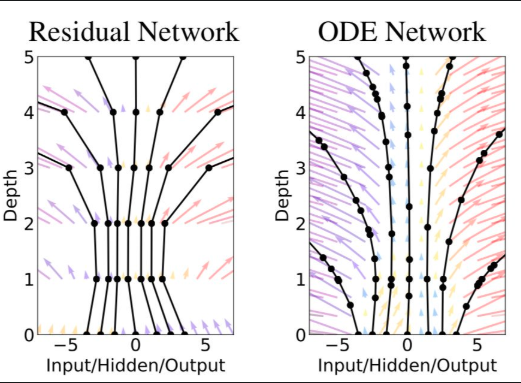
\includegraphics[scale=0.7]{resnetvsodenet.png}
\end{center}


%TODO dire que resnet peut calculer par exemple $y=x^2$ mais pas ode net qui lui ne peut apprendre que des transformations bijectives : lien avec les conditions pour avoir une solution à une ode?


\end{document}